\chapter{Introducere}

Un subdomeniu al inteligenței artificiale care a captat interesul publicului, al sectorului privat și al instituțiilor guvernamentale este vederea artificială. În ultimii ani au fost înregistrate progrese semnificative atât în dezvoltarea de noi metode utilizate în vederea artificială, cât și al capacității de procesare a datelor și implementare a acestor noi algoritmi. Vederea artificială are un rol bine stabilit într-o gamă variată de cazuri, cum ar fi robotica, securitatea unei instituții, industria \textit{software} (recunoaștere facială, realitate augmentată) și, cel mai important pentru lucrarea de față, medicina și accesibilitatea.

Această lucrare își propune să contribuie la apropierea de persoanele care prezintă deficiențe de auz și/sau vorbire. Având în vedere importanța integrării acestora și nevoia de a ușura interacțiunea, vizăm să reducem bariera apărută în comunicare. Aplicația dezvoltată sprijină indivizii care doresc fie să traducă literele exprimate cu ajutorul mâinilor, fie să învețe sau să exerseze alfabetul limbajului american al semnelor (în engl. \textit{American Sign Language} - ASL).

Pentru a ne atinge scopul, utilizăm tehnici de \textit{deep learning} pentru antrenarea unui model bazat pe o rețea neuronală convoluțională (în engl. Convolutional Neural Network - CNN), reprezentând nucleul aplicației mobile Android folosite de utilizator. Aplicația reprezintă interfața prin care utilizatorul interacționează cu rețeaua neuronală antrenată. Aceasta transmite modelului cadrele capturate cu ajutorul camerei dispozitivului, modelul le analizează și returnează rezultatele detecției.

În căutarea unui set de date potrivit pentru antrenare, am observat că majoritatea seturilor de date privind alfabetul ASL conțineau doar imagini similare, fie ca fundal, fie ca poziție a mâinii, făcând dificilă antrenarea unui model asupra unui singur set de date. Pentru a depăși această problemă, s-a optat pentru combinarea mai multor surse, pentru a ajuta modelul în generalizare. Un set de date a fost creat special pentru acest studiu prin înregistrarea video a autorului lucrării și a unui voluntar, trei seturi au fost preluate de pe \textbf{Youtube} \cite{youtube_dataset0, youtube_dataset1, youtube_dataset2}, cinci au fost preluate de pe \textbf{Kaggle} \cite{kaggle_dataset0, kaggle_dataset1, kaggle_dataset2, kaggle_dataset3, kaggle_dataset4}, iar restul de cinci din articole științifice \cite{article_dataset0, article_dataset1, article_dataset2, article_dataset3, article_dataset4}, integrând un total de 14 surse.

Pentru început, am remarcat faptul că seturile de date originale conțineau imagini cu litere aparținând mai multor dialecte ale alfabetului ASL. Prin urmare, materialul oferit de \textit{American Society for Deaf Children} (ASDC), ilustrat în Figura~\ref{fig:exemplu_litere_fingerspell}, servește drept referință în filtrarea manuală a imaginilor.

\begin{figure}[H]
  \centering
  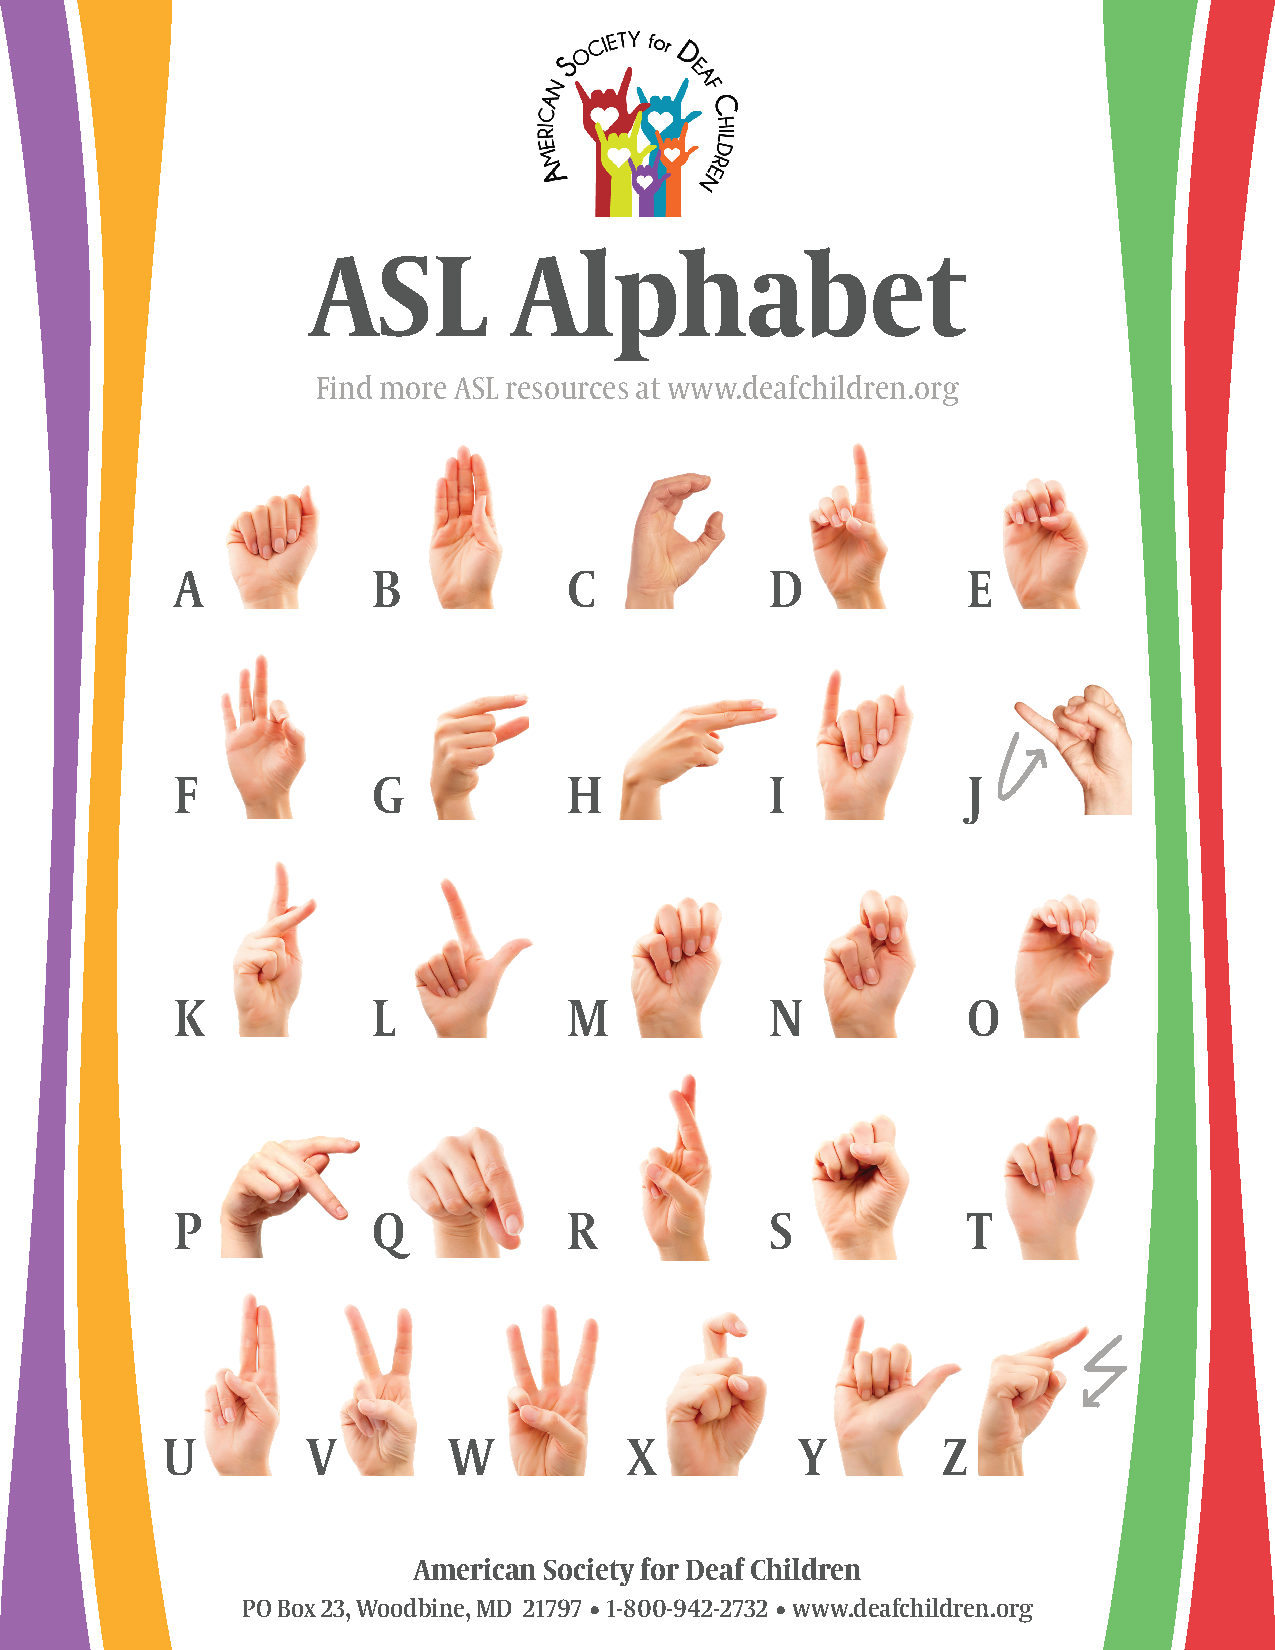
\includegraphics[width=0.5\textwidth]{images/2-recunoasterea-asl/ASL-Alphabet-ASDC.pdf}
  \caption[Alfabetul ASL]{\textbf{Alfabetul ASL}. \textit{Imagine preluată de pe website-ul ASDC \cite{asl_alphabet_chart}. Fiecare palmă reprezintă o literă din alfabet. J și Z presupun mișcare, așadar săgețile indică forma mișcării.}}
  \label{fig:exemplu_litere_fingerspell}
\end{figure}

În cazul în care unul sau mai multe dialecte diferite de cel ilustrat în Figura~\ref{fig:exemplu_litere_fingerspell} aveau reprezentativitate consistentă, s-a decis păstrarea acestora, întrucât modelul este capabil să învețe diferite dialecte pentru o literă, cât timp „vede” destule exemple. Un caz de acest fel poate fi observat în Figura~\ref{fig:p_2_dialecte}.

\begin{figure}[H]
  \centering
  \begin{subfigure}{0.3\textwidth}
    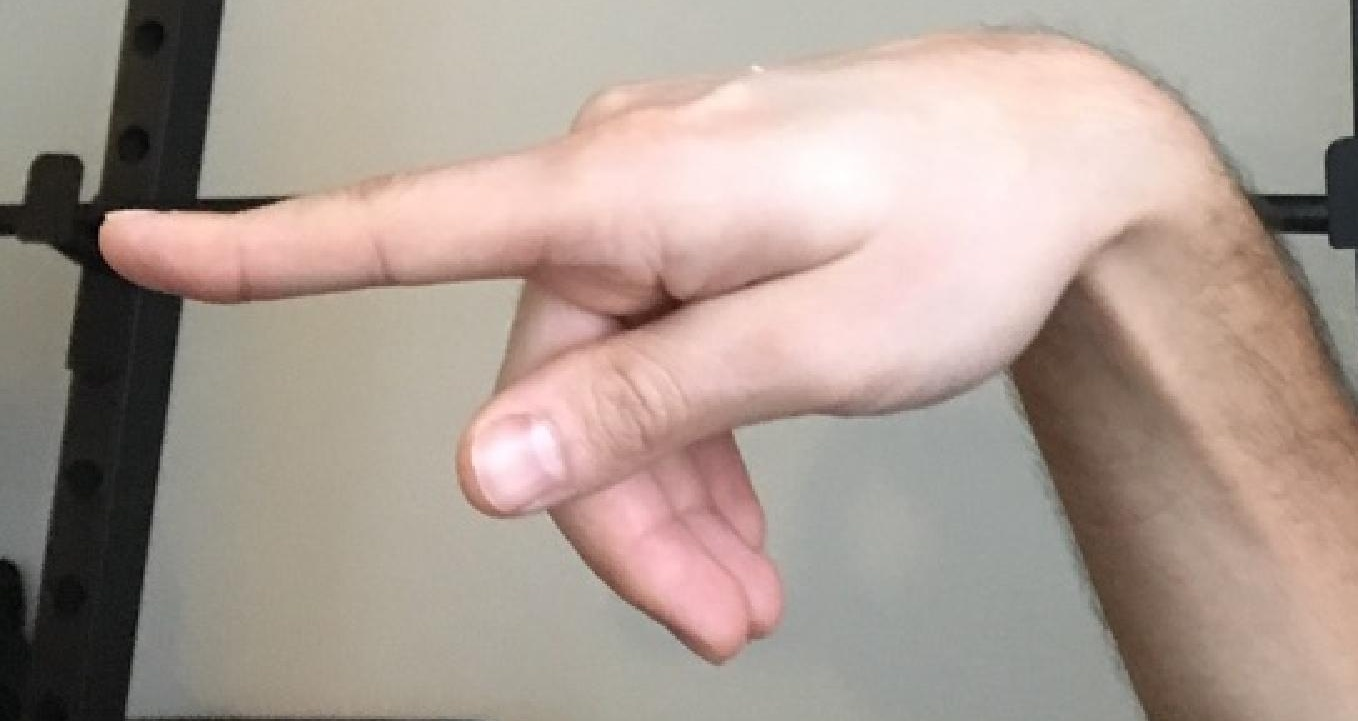
\includegraphics[width=\linewidth]{images/2-recunoasterea-asl/p_dialect1.png}
    \caption{}
    \label{fig:img1}
  \end{subfigure}
    \hspace{0.1\textwidth}
  \begin{subfigure}{0.3\textwidth}
    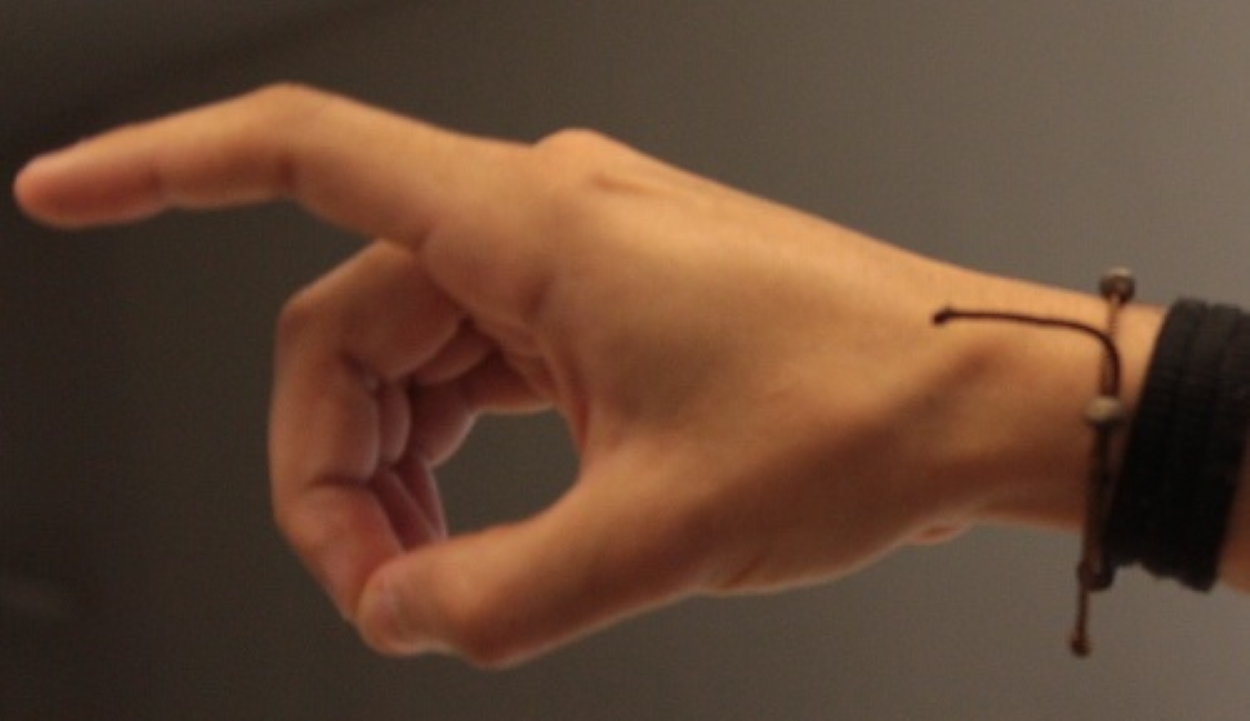
\includegraphics[width=\linewidth]{images/2-recunoasterea-asl/p_dialect2.png}
    \caption{}
    \label{fig:img2}
  \end{subfigure}
  \caption[Dialecte pentru litera P]{\textbf{Dialecte pentru litera P}. \textit{Ambele imagini ilustrează aceeași literă, P, și exemplifică două dialecte diferite, provenind din surse distincte.}}
  \label{fig:p_2_dialecte}
\end{figure}
Literele J și Z au fost eliminate deoarece presupun mișcarea mâinii, iar aplicația noastră analizează un singur cadru independent.


Câte un exemplu sugestiv pentru fiecare literă din setul de date final poate fi analizat în Figura~\ref{fig:ex_per_litera}.
\captionsetup[subfigure]{labelformat=empty}

\begin{figure}[H]

  \centering

  \begin{subfigure}{0.1\textwidth}
    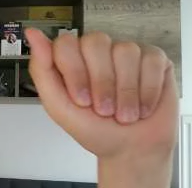
\includegraphics[width=2cm, height=2cm, keepaspectratio=false]{images/7-anexe/a_ex10.png}
    \caption{A}
  \end{subfigure}\hspace{1cm}
  \begin{subfigure}{0.1\textwidth}
    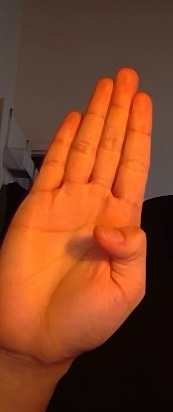
\includegraphics[width=2cm, height=2cm, keepaspectratio=false]{images/7-anexe/b_ex1.jpg}
    \caption{B}
  \end{subfigure}\hspace{1cm}
  \begin{subfigure}{0.1\textwidth}
    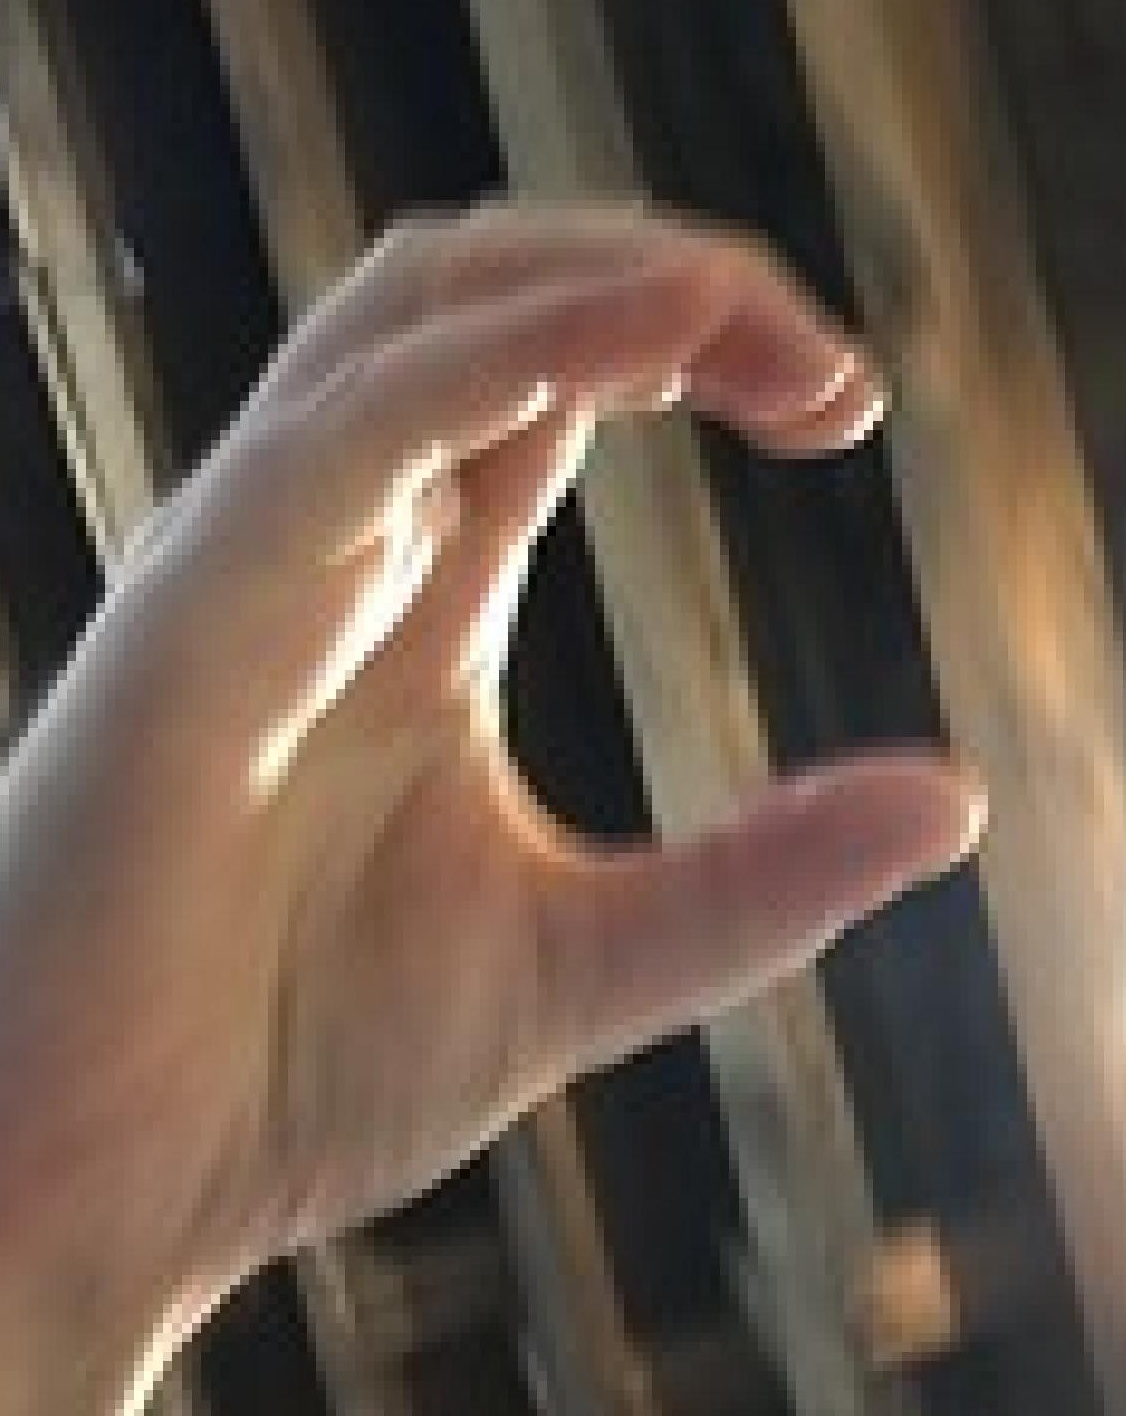
\includegraphics[width=2cm, height=2cm, keepaspectratio=false]{images/7-anexe/c_ex1.jpg}
    \caption{C}
  \end{subfigure}\hspace{1cm}

  

  \begin{subfigure}{0.1\textwidth}
    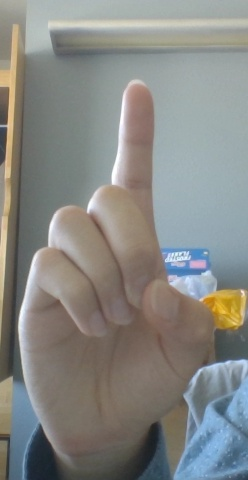
\includegraphics[width=2cm, height=2cm, keepaspectratio=false]{images/7-anexe/d_ex1.jpg}
    \caption{D}
  \end{subfigure}\hspace{1cm}
  \begin{subfigure}{0.1\textwidth}
    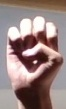
\includegraphics[width=2cm, height=2cm, keepaspectratio=false]{images/7-anexe/e_ex1.jpg}
    \caption{E}
  \end{subfigure}\hspace{1cm}
  \begin{subfigure}{0.1\textwidth}
    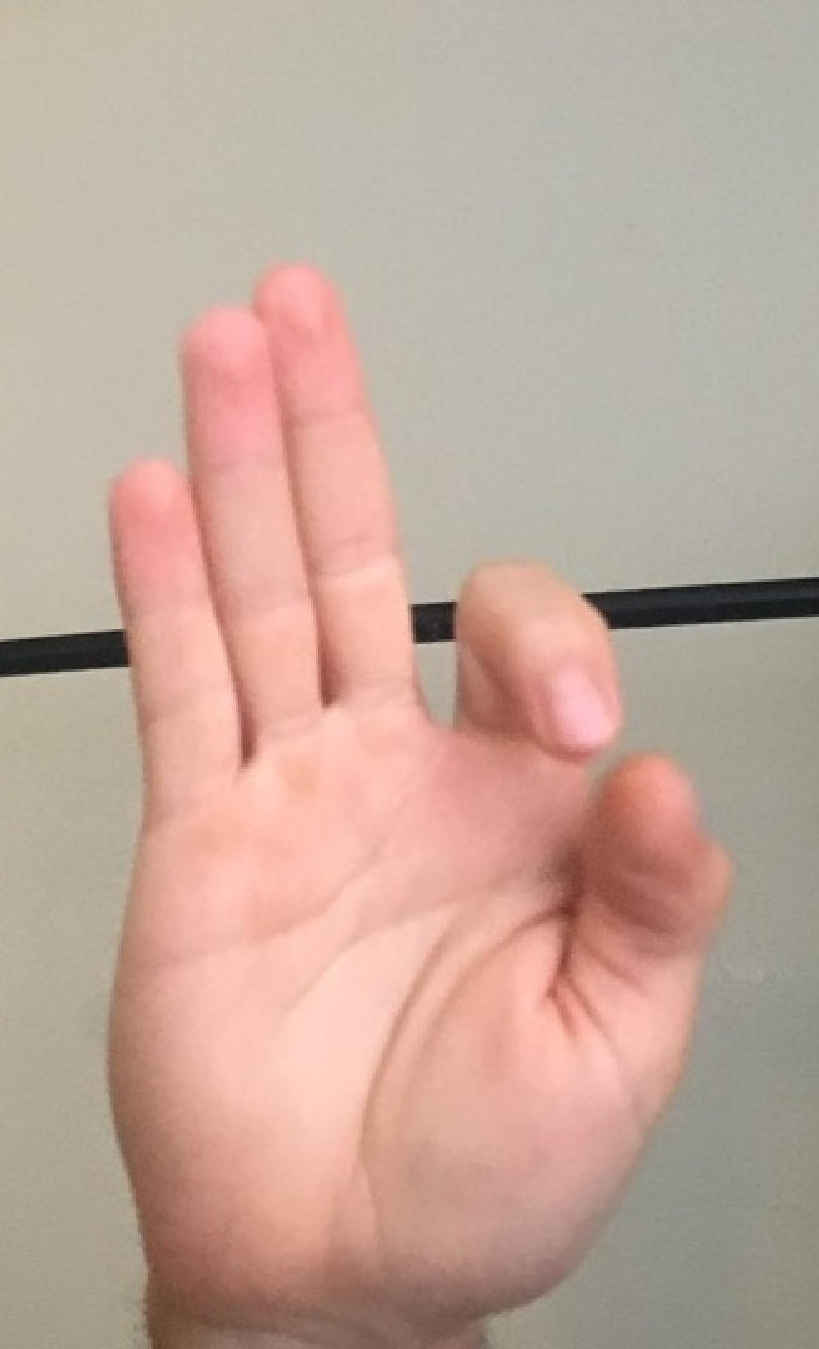
\includegraphics[width=2cm, height=2cm, keepaspectratio=false]{images/7-anexe/f_ex1.jpg}
    \caption{F}
  \end{subfigure}\hspace{1cm}

  

  \begin{subfigure}{0.1\textwidth}
    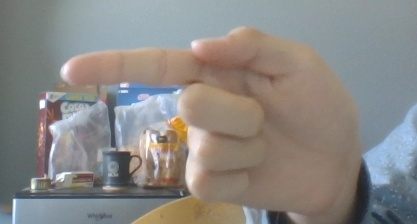
\includegraphics[width=2cm, height=2cm, keepaspectratio=false]{images/7-anexe/g_ex1.jpg}
    \caption{G}
  \end{subfigure}\hspace{1cm}
  \begin{subfigure}{0.1\textwidth}
    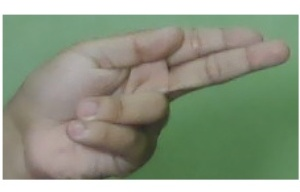
\includegraphics[width=2cm, height=2cm, keepaspectratio=false]{images/7-anexe/h_ex1.jpg}
    \caption{H}
  \end{subfigure}\hspace{1cm}
  \begin{subfigure}{0.1\textwidth}
    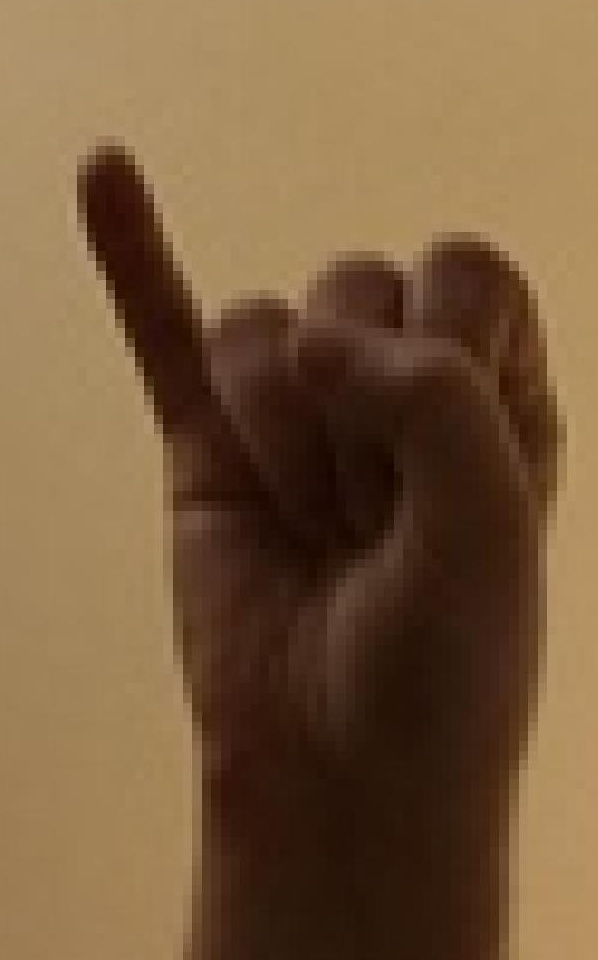
\includegraphics[width=2cm, height=2cm, keepaspectratio=false]{images/7-anexe/i_ex1.jpg}
    \caption{I}
  \end{subfigure}\hspace{1cm}
    
    \begin{subfigure}{0.1\textwidth}
    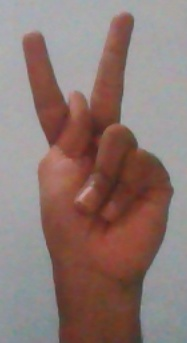
\includegraphics[width=2cm, height=2cm, keepaspectratio=false]{images/7-anexe/k_ex1.jpg}
    \caption{K}
  \end{subfigure}\hspace{1cm}
  \begin{subfigure}{0.1\textwidth}
    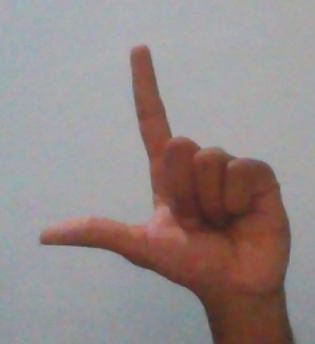
\includegraphics[width=2cm, height=2cm, keepaspectratio=false]{images/7-anexe/l_ex1.jpg}
    \caption{L}
  \end{subfigure}\hspace{1cm}
  \begin{subfigure}{0.1\textwidth}
    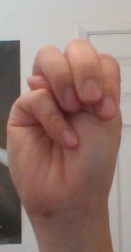
\includegraphics[width=2cm, height=2cm, keepaspectratio=false]{images/7-anexe/m_ex1.jpg}
    \caption{M}
  \end{subfigure}\hspace{1cm}

  

  \begin{subfigure}{0.1\textwidth}
    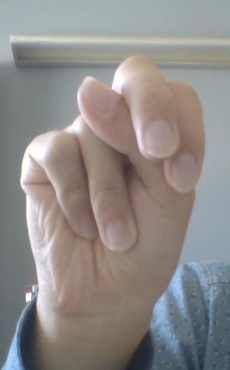
\includegraphics[width=2cm, height=2cm, keepaspectratio=false]{images/7-anexe/n_ex1.jpg}
    \caption{N}
  \end{subfigure}\hspace{1cm}
  \begin{subfigure}{0.1\textwidth}
    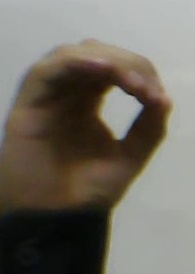
\includegraphics[width=2cm, height=2cm, keepaspectratio=false]{images/7-anexe/o_ex1.jpg}
    \caption{O}
  \end{subfigure}\hspace{1cm}
  \begin{subfigure}{0.1\textwidth}
    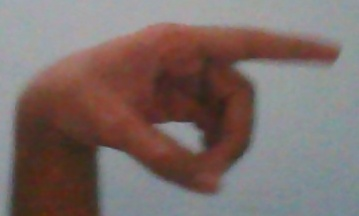
\includegraphics[width=2cm, height=2cm, keepaspectratio=false]{images/7-anexe/p_ex1.jpg}
    \caption{P}
  \end{subfigure}\hspace{1cm}

  

  \begin{subfigure}{0.1\textwidth}
    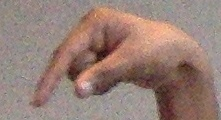
\includegraphics[width=2cm, height=2cm, keepaspectratio=false]{images/7-anexe/q_ex1.jpg}
    \caption{Q}
  \end{subfigure}\hspace{1cm}
  \begin{subfigure}{0.1\textwidth}
    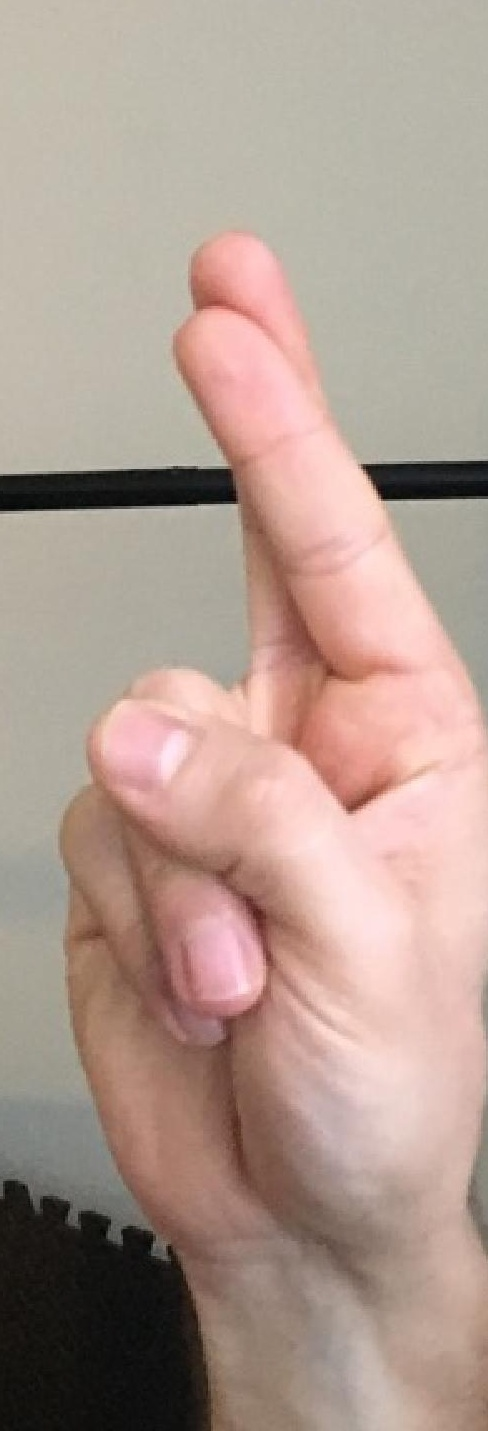
\includegraphics[width=2cm, height=2cm, keepaspectratio=false]{images/7-anexe/r_ex1.jpg}
    \caption{R}
  \end{subfigure}\hspace{1cm}
  \begin{subfigure}{0.1\textwidth}
    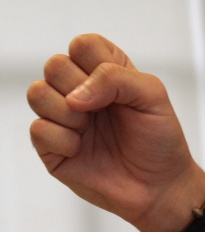
\includegraphics[width=2cm, height=2cm, keepaspectratio=false]{images/7-anexe/s_ex1.JPG}
    \caption{S}
  \end{subfigure}\hspace{1cm}

    \begin{subfigure}{0.1\textwidth}
    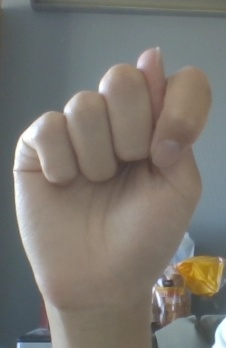
\includegraphics[width=2cm, height=2cm, keepaspectratio=false]{images/7-anexe/t_ex1.jpg}
    \caption{T}
  \end{subfigure}\hspace{1cm}
  \begin{subfigure}{0.1\textwidth}
    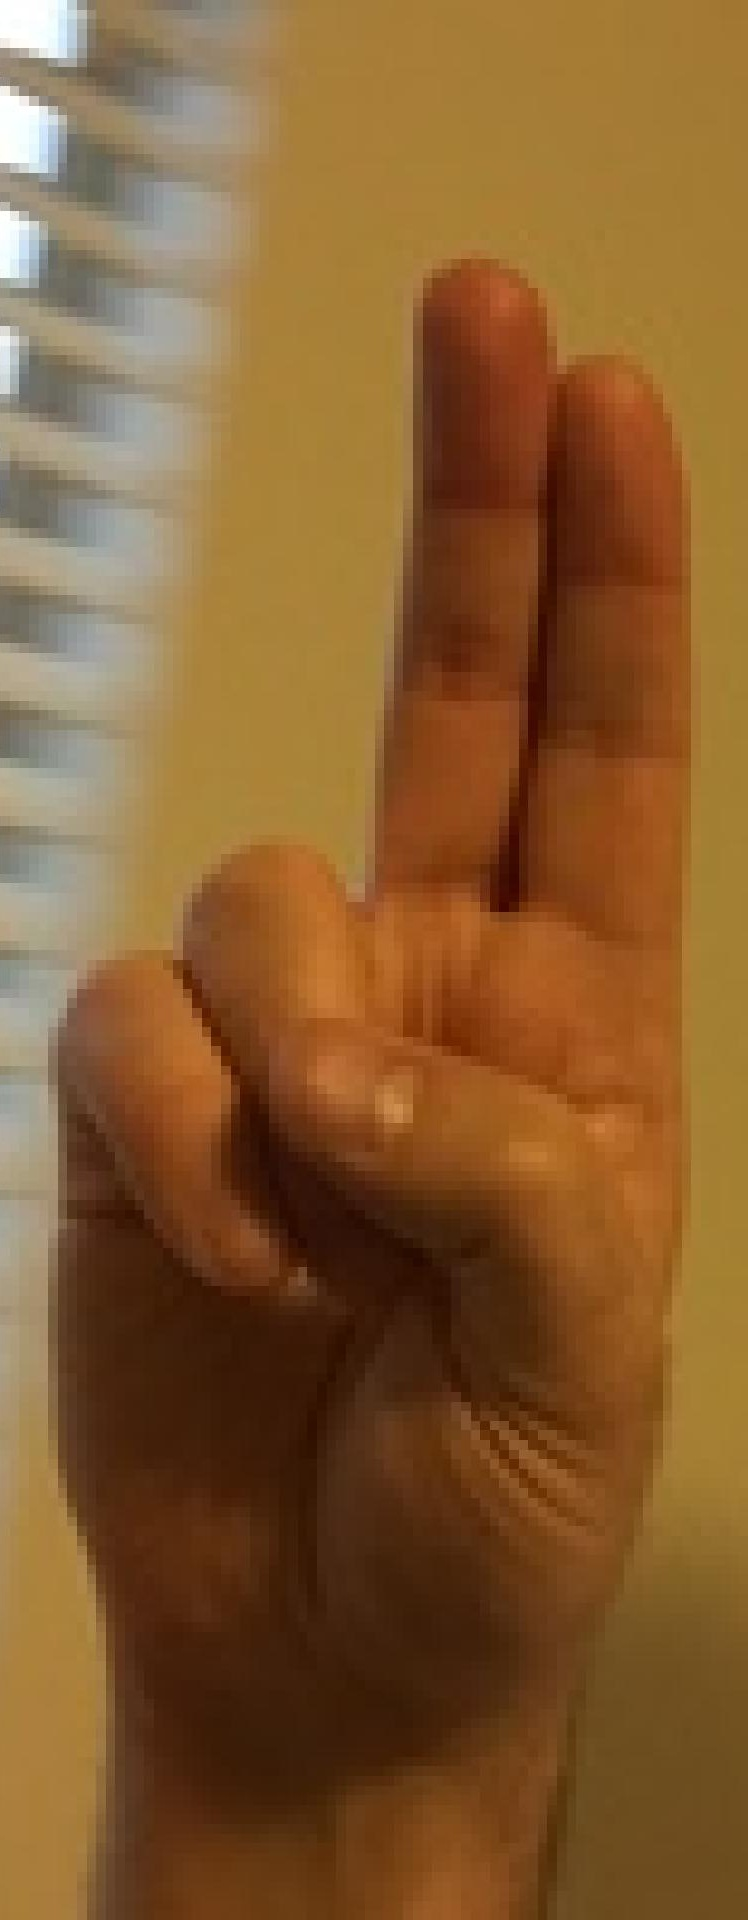
\includegraphics[width=2cm, height=2cm, keepaspectratio=false]{images/7-anexe/u_ex1.jpg}
    \caption{U}
  \end{subfigure}\hspace{1cm}
  \begin{subfigure}{0.1\textwidth}
    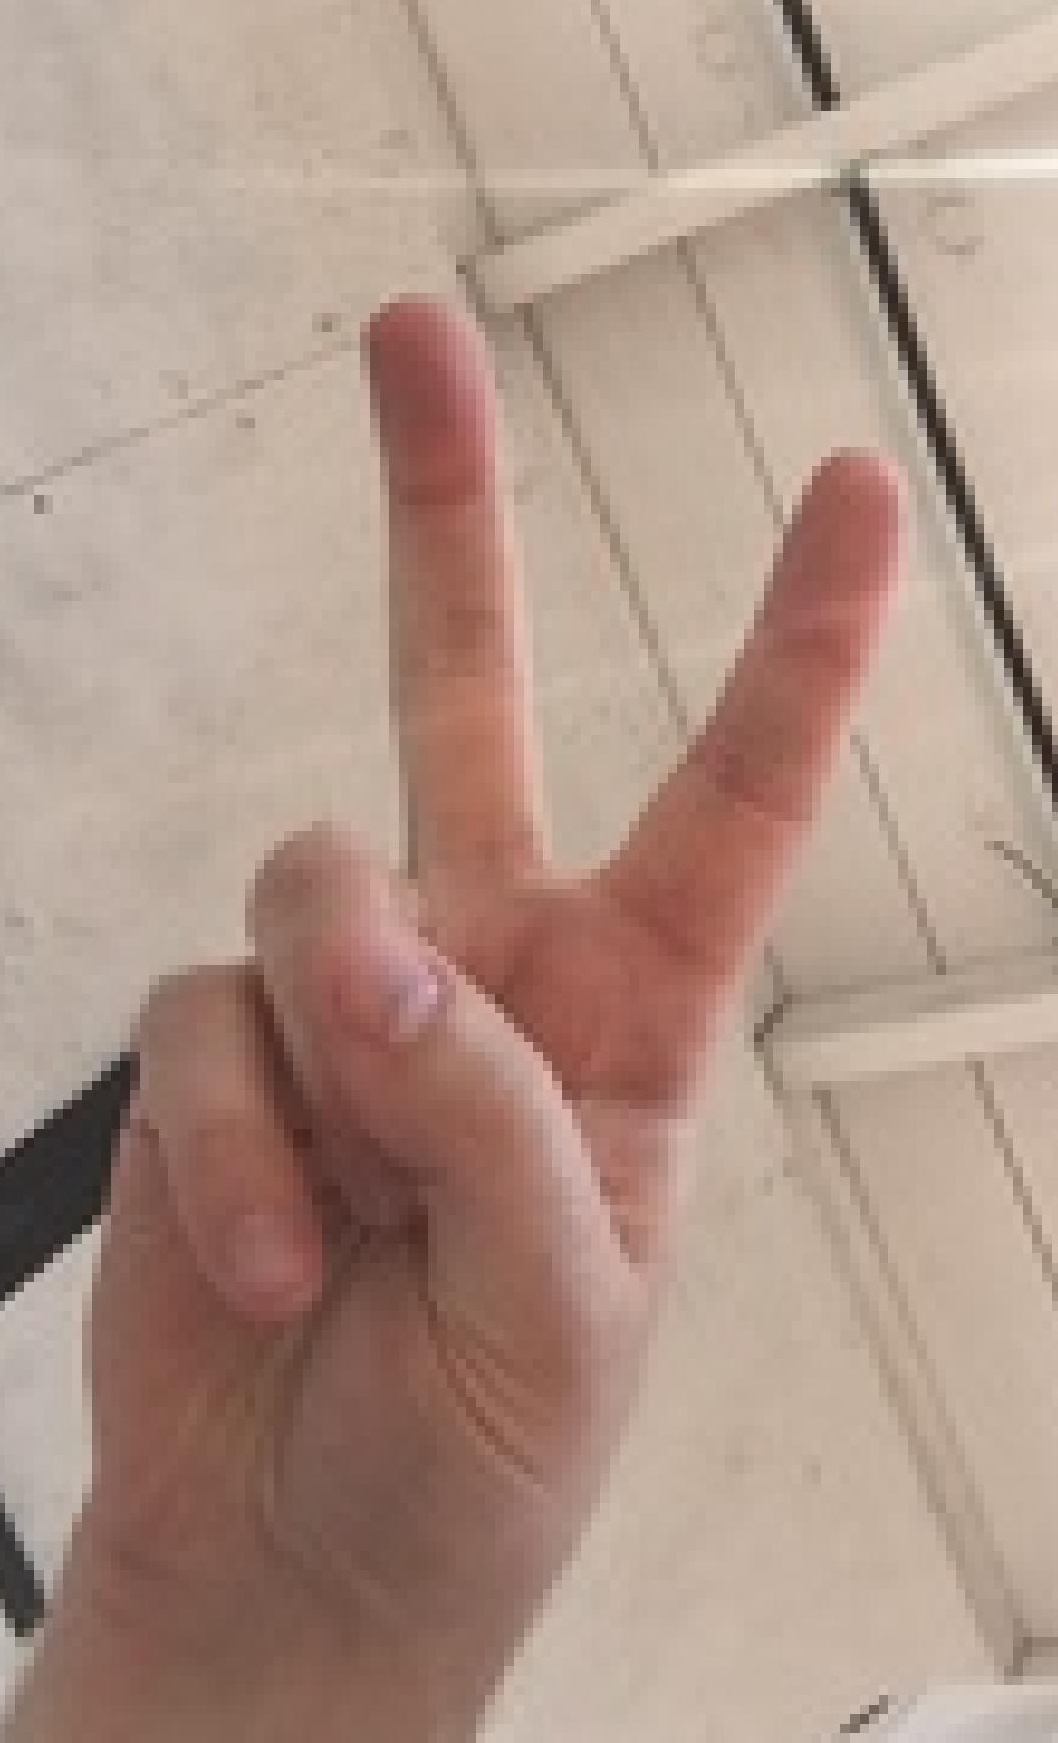
\includegraphics[width=2cm, height=2cm, keepaspectratio=false]{images/7-anexe/v_ex1.jpg}
    \caption{V}
  \end{subfigure}\hspace{1cm}

  

  \begin{subfigure}{0.1\textwidth}
    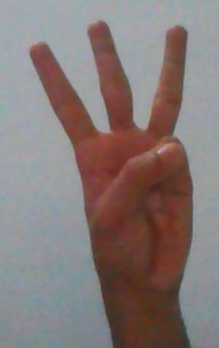
\includegraphics[width=2cm, height=2cm, keepaspectratio=false]{images/7-anexe/w_ex1.jpg}
    \caption{W}
  \end{subfigure}\hspace{1cm}
  \begin{subfigure}{0.1\textwidth}
    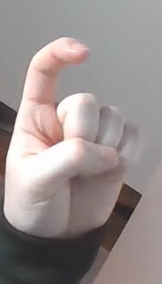
\includegraphics[width=2cm, height=2cm, keepaspectratio=false]{images/7-anexe/x_ex1.png}
    \caption{X}
  \end{subfigure}\hspace{1cm}
  \begin{subfigure}{0.1\textwidth}
    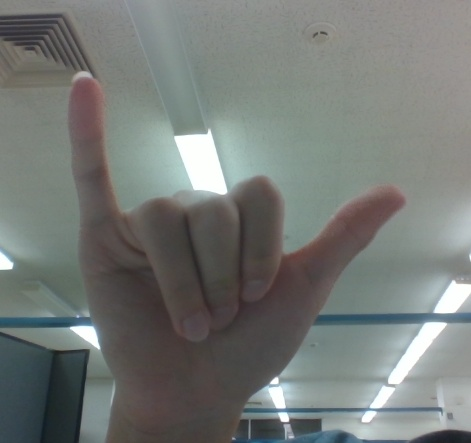
\includegraphics[width=2cm, height=2cm, keepaspectratio=false]{images/7-anexe/y_ex1.jpg}
    \caption{Y}
  \end{subfigure}\hspace{1cm}
  \caption[Literele din setul de date.]{\textbf{Literele din setul de date.} \textit{Ilustrăm câte un exemplu ales aleator, pentru fiecare clasă. Litera situată sub fiecare imagine reprezintă clasa corespunzătoare.}}
  \label{fig:ex_per_litera}
\end{figure}
\captionsetup[subfigure]{labelformat=parens, labelsep=space}

Lucrarea de față este structurată în trei capitole principale, după cum urmează:
\begin{enumerate}
    \item \textbf{Recunoașterea alfabetului ASL} - în acest capitol explicăm procesul care a stat la baza creării setului de date, preprocesarea imaginilor, arhitectura modelului și procesul de antrenare al acestuia. În final, oferim o evaluare experimentală în care analizăm arhitecturile și strategiile nereușite care au contribuit la construirea arhitecturii finale.
    \item \textbf{Aplicația mobilă și infrastructura aplicației} - în acest capitol prezentăm ecranele principale ale aplicației Android, continuând cu o analiză a logicii aplicației și a capacității serverului.
    \item \textbf{Direcții viitoare și concluzii} - în acest ultim capitol recapitulăm procesul științific, analizăm limitările și lipsurile aplicației, posibile soluții privind limitele menționate și oferim direcții viitoare de dezvoltare.
\end{enumerate}